\section{Vergleich beider Systeme} \label{sec:Vergleich}
In \autoref{fig:Bild2} ist die Übersicht der notwendigen Simulationsstruktur dargestellt. Aus der Übersicht geht hervor, dass beide Systeme unterschiedliche Eingänge besitzen und somit ein direkter Vergleich ohne entsprechende Berücksichtigung der Linearisierungsvorschriften unmöglich ist. Das linearisierte Modell verwendet als Eingang im Gegensatz zum nichtlinearen Modell eine Differenz $\Delta d$. Dies folgt aus \autoref{eq:Gleichung15}. Die Variable $d_{\mathrm{dyn}}$ sei gleich der Konstante $d$. Die Strukturen des nichtlinearen und des linearen Modells sind zur Information in \autoref{fig:Bild4} und \autoref{fig:Bild3} visualisiert.

\begin{figure}[H]
   \centering
   \fbox{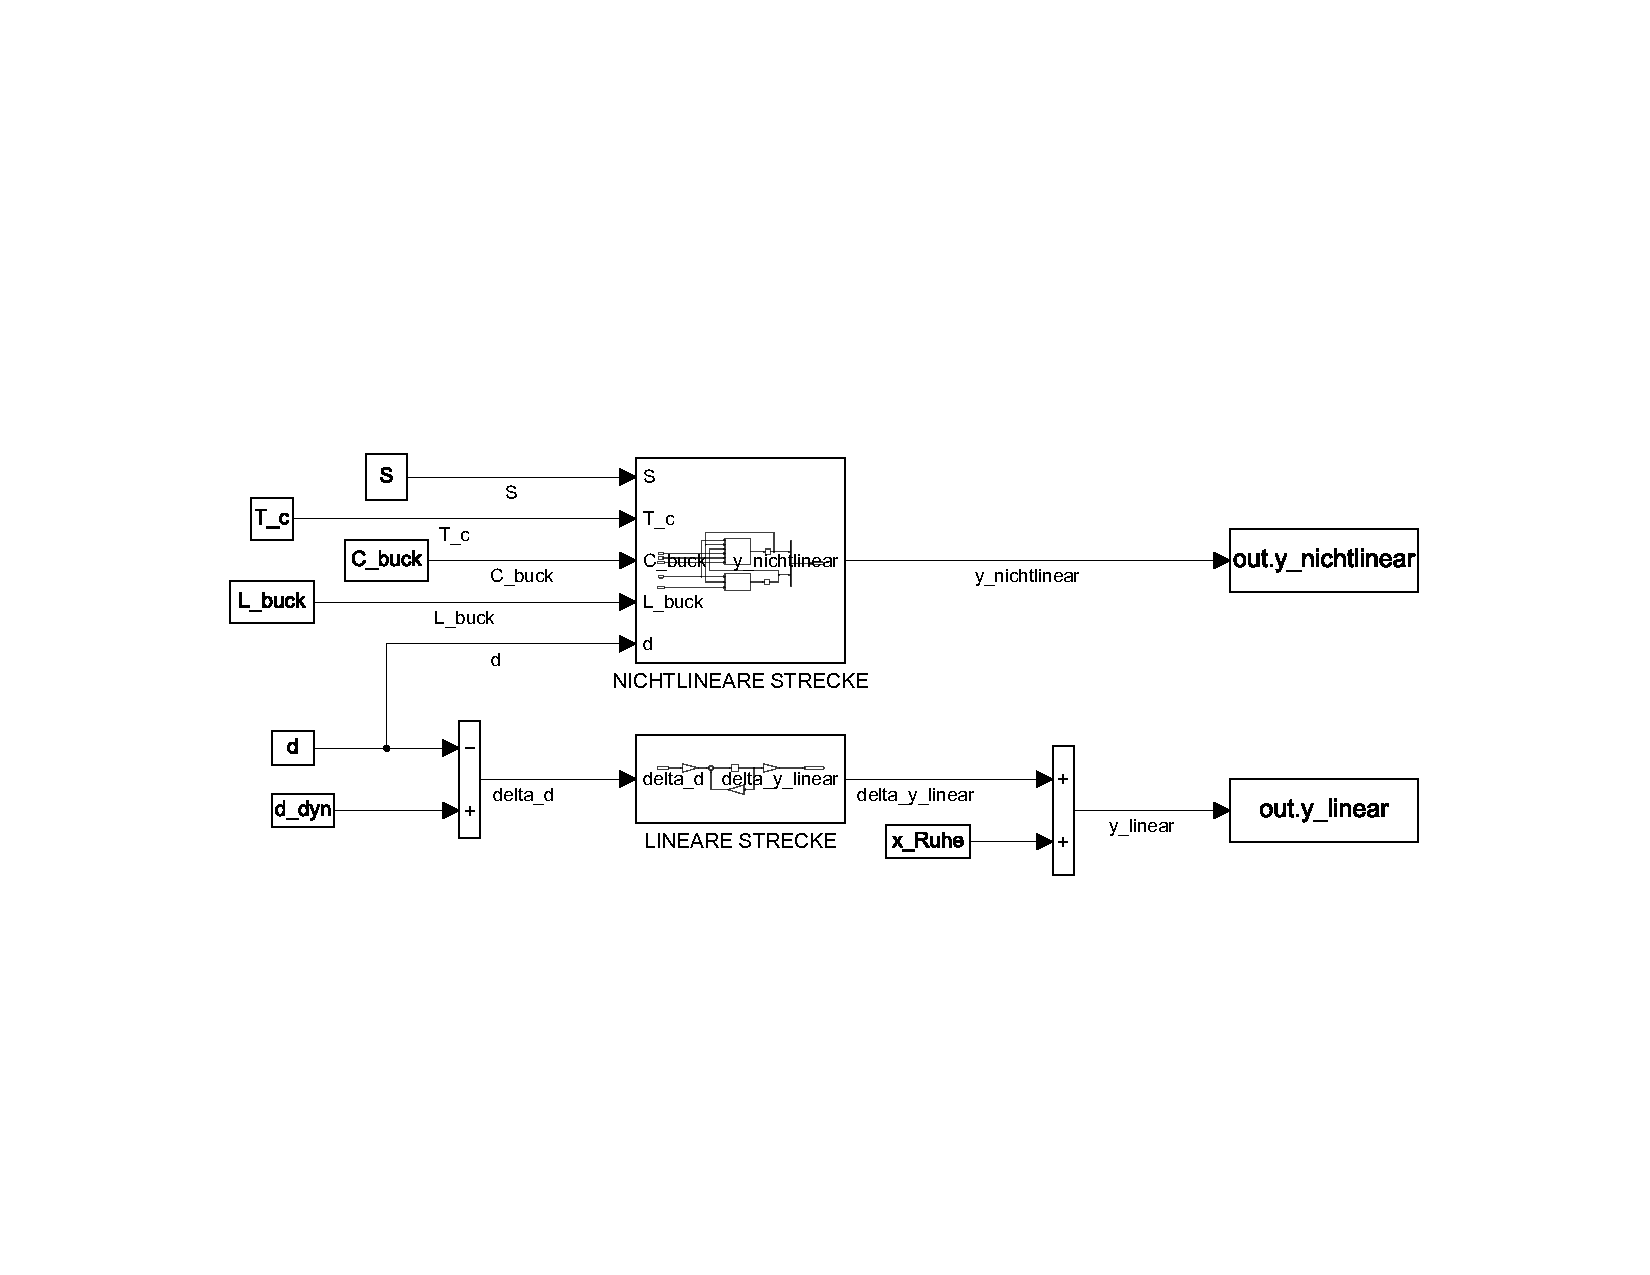
\includegraphics[width=0.9\textwidth]{Bilder/4_vergleich/Vergleich_linear_nichtlinear_Uebersicht.pdf}}
   \caption[Übersicht der Simulationsstruktur]{Übersicht der Simulationsstruktur}
   \label{fig:Bild2}
\end{figure}

\begin{figure}[H]
   \centering
   \fbox{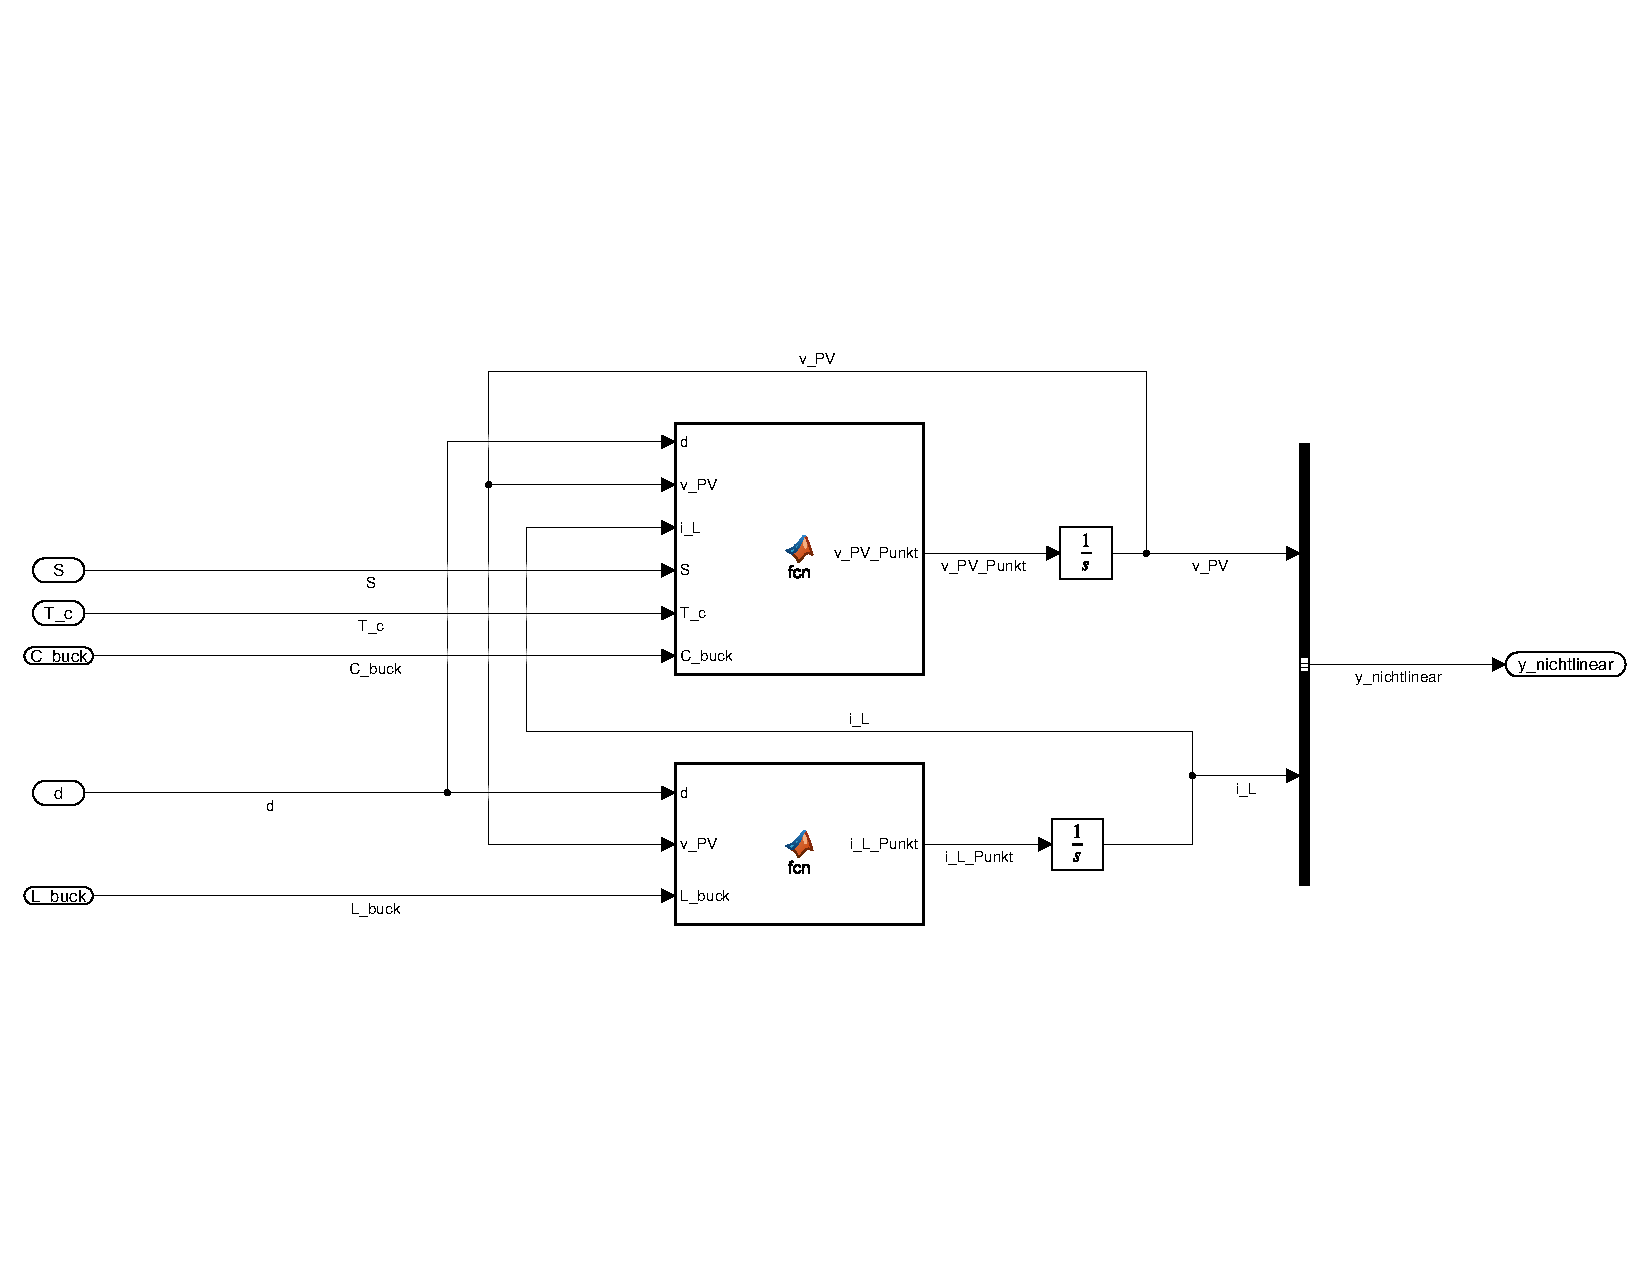
\includegraphics[width=0.9\textwidth]{Bilder/4_vergleich/Vergleich_linear_nichtlinear_Nichtlineare_Strecke.pdf}}
   \caption[Nichtlineare Strecke]{Nichtlineare Strecke}
   \label{fig:Bild3}
\end{figure}

\begin{figure}[H]
   \centering
   \fbox{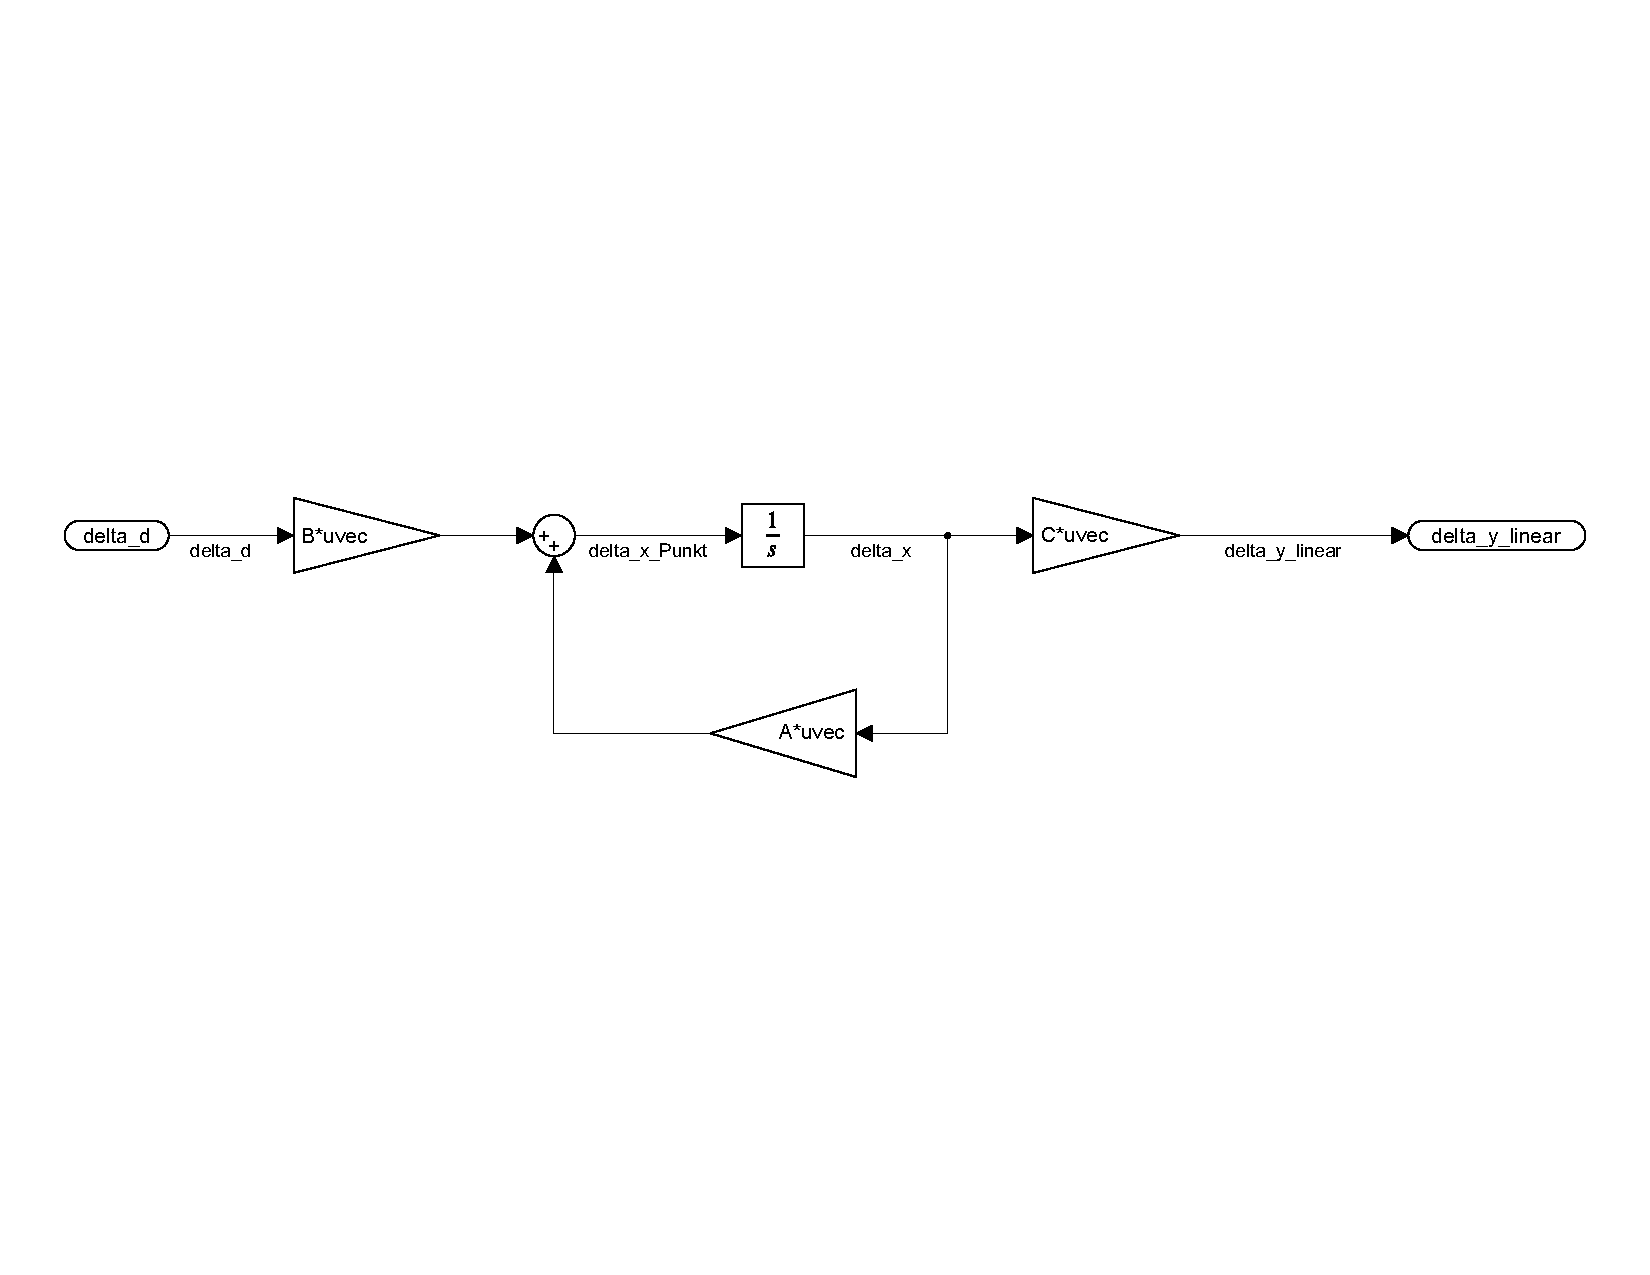
\includegraphics[width=0.9\textwidth]{Bilder/4_vergleich/Vergleich_linear_nichtlinear_Lineare_Strecke.pdf}}
   \caption[Lineare Strecke]{Lineare Strecke}
   \label{fig:Bild4}
\end{figure}

Um das lineare mit dem nichtlinearen Modell zu vergleichen, werden gemäß \autoref{sec:Zustandsraummodell} zu den Zuständen $\Delta \underline{x}$ die Ruhelagen $\underline{x}^*$ aus \autoref{eq:Gleichung11} addiert. Aus der \autoref{fig:Bild5} und \autoref{fig:Bild6} geht hervor, dass das nichtlineare System aufgund der Nichtlinearität zu schwingen anfängt, jedoch nach ca. 0.15s erwartungsgemäß in die Ruhelagen, d.h. in den MPP, pendelt. Die implementierten Systeme weisen für kleine Abweichungen von der Ruhelagen mit steigender Zeit $"t"$ selbiges Verhalten auf.

\begin{figure}[H]
   \centering
   \fbox{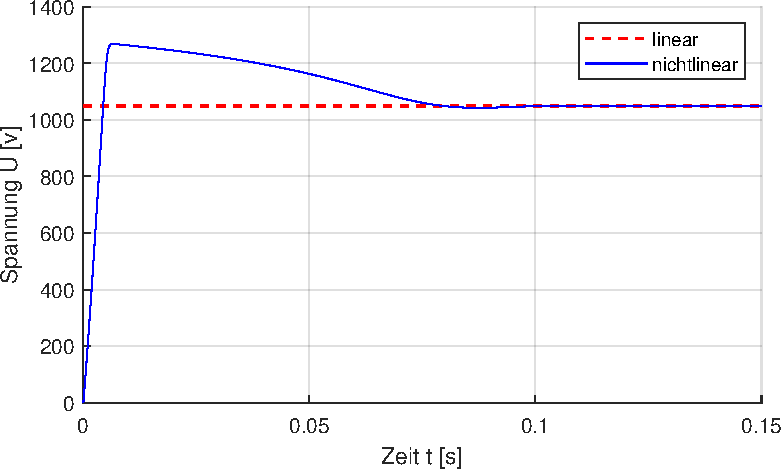
\includegraphics[width=0.9\textwidth]{Bilder/4_vergleich/linear_nichtlinear_vergleich_v_PV.pdf}}
   \caption[Vergleich der Spannungen $v_{\mathrm{PV}}$]{Vergleich der Spannungen $v_{\mathrm{PV}}$}
   \label{fig:Bild5}
\end{figure}

\begin{figure}[H]
   \centering
   \fbox{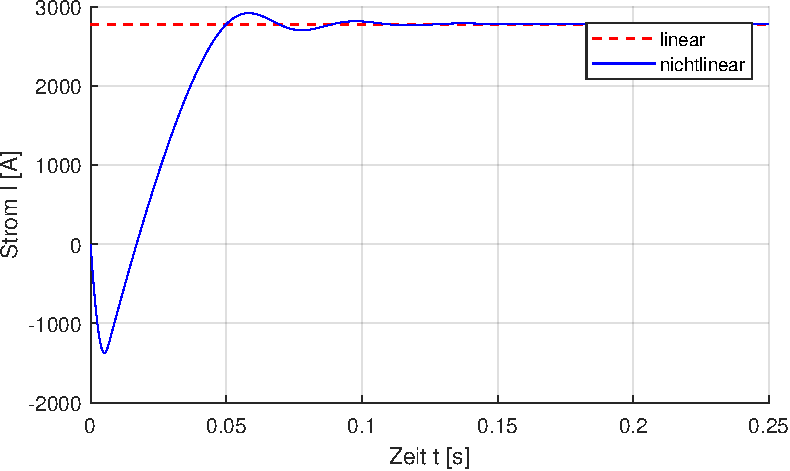
\includegraphics[width=0.9\textwidth]{Bilder/4_vergleich/linear_nichtlinear_vergleich_i_L.pdf}}
   \caption[Vergleich der Ströme $i_{\mathrm{L}}$]{Vergleich der Ströme $i_{\mathrm{L}}$}
   \label{fig:Bild6}
\end{figure}
